\chapter{Di-$b$-jet Search: Limit Setting}
\label{sec:lim}

%Specifically, what was found was that the probability of obtaining a data-set with an excess similar to the one observed
%under the assumption that there is new physics was above a certain threshold.
%This lead to the conclusion that there is no evidence of BSM physics in the di-$b$-jet spectra.

In Chapter~\ref{sec:bkg} it was shown that there is no evidence of new physics in the di-$b$-jet spectra considered.
However, it is also useful to quantify what this result means in the context
of the signal models that we are searching for.
Specifically, we can estimate the degree of belief that a signal model is true given the di-$b$-jet spectra that have been observed.
If the degree of belief of a specific model is less than a certain threshold it is said that this model is excluded.
This process is known as limit setting.

In this Chapter:
Section~\ref{sec:lim-strat} will describe the limit setting strategy used,
Section~\ref{sec:lim-syst} will discuss the systematic uncertainties considered
and in Section~\ref{sec:lim-summer} and Section~\ref{sec:lim-full}
the results of the limit setting procedure for the various data-sets considered are shown.

\section{Bayesian Limits}
\label{sec:lim-strat}

In this analysis a Bayesian limit setting approach is used~\cite{lim-bayes}.
For limit setting, one considers a hypothesis that the di-$b$-jet events are produced by a combination of 
the QCD background, which has been modelled by the background fit from the previous chapter,
and some new physics process 
which produces $\mu$ events according to some template shape in~\mjj.
This signal plus background hypothesis is denoted by the symbol $H_\mu$.

Now let us consider this hypothesis in the context of the data, denoted by $D$,
which in this case is one of our observed di-$b$-jet spectra.
For the hypothesis, $H_\mu$, the probability of producing the data is known as the ``likelihood''.
If, in each~\mjj~bin, the model predicts
$s_i(\mu)$ signal events, $b_i$ background events and $n_i$ events were observed in data.
Then, by only considering statistical uncertainties, the likelihood for a given value of $\mu$ is given by
\begin{equation}
  \Like (\mu,D) = P(D \mid \mu) =  \Pi_i \frac{(s_i(\mu)+b_i)^{n_i}~e^{-(s_i(\mu)+b_i)}}{n_i!}
\end{equation}
where the product is over all~\mjj~bins.

\noindent
Then, one can employ Bayes' theorem which states that
\begin{equation}
  P(A \mid B) = \frac{P(B \mid A) \, P(A)}{P(B)}
\end{equation}
to obtain the probability density function of $\mu$ given the observed di-$b$-jet spectrum,
\begin{equation}
  P(\mu \mid D) = \frac{ P(D \mid \mu) \, \Pi( \mu ) }{ \Pi( D ) }
  \label{eq:lim-conf_statOnly}
\end{equation}
This quantity, known as the posterior, is an expression of our confidence in the hypothesis
$H_\mu$ for any particular value of $\mu$.

The $\Pi( \mu )$ term in the posterior %Equation~\ref{eq:lim-conf_statOnly}
is called the signal prior
and gives the probability density of $\mu$ before the experiment took place.
For this experiment a flat signal prior was chosen
\footnote{Flat from $\mu$ = 0 to the value of $\mu$ where the
likelihood has fallen to $10^{-5}$ of the optimal likelihood value.}
which represents ignorance to the size of the signal before the experiment.
The $\Pi(D)$ term does not depend on $\mu$ and as such can be considered as a normalisation term.

However, to accurately represent a true degree of belief in a model one must consider systematic uncertainties,
which are uncertainties in the model's predictions.
The systematic uncertainties considered in this analysis are listed below in Section~\ref{sec:lim-syst}.
The systematic uncertainties are incorperated by making $s_i$ and $b_i$ a function of a set of
nuisance parameters, $\vec{\theta}$, where each nuissance parameter models the effect of a systematic uncertainty.
Therefore likelihood becomes a function of the nuisance parameters
\begin{equation}
  \Like (\mu,D,\vec{\theta}) = P(D \mid \mu, \vec{\theta} ) 
\end{equation}
The effect of the systematic uncertainties are then propagated to the posterior. %Equation~\ref{eq:lim-conf_statOnly}.
To do this a prior is introduced for each the nuisance parameters, given by $\Pi(\vec{\theta})$,
that describes the probability distribution of the nuissance parameters.
Then, by integrating over the nuisance parameters,
one obtains the probability density function for $\mu$ that includes the systematic uncertainties
\begin{equation}
  P(\mu \mid D) \propto \int d \vec{\theta} \, \Like (\mu, D, \vec{\theta} ) \, \Pi( \mu )  \, \Pi(\vec{\theta})
  \label{eq:lim-conf_syst}
\end{equation}
One can calculate the likelihoods for the data,
perform the integral over nuisance parameters
and then normalise to calculate the probability density of $\mu$
\footnote{This integral is performed using a Monte-Carlo Markov chain using the Bayesian Analysis Toolkit.
 Full details on the implementation can be found here~\cite{det-thesis_kate}.}.

Using the posterior calculated from Equation~\ref{eq:lim-conf_syst},
the 95\% confidence level upper limit of $\mu$, denoted by $\mu_{up}\,$,
is calculated using the expression
\begin{equation}
\int_0^{\mu_{up}} P(\mu \mid D)~=~0.95
\end{equation}
The 95\% confidence upper limit
defines a confidence region ($0 < \mu < \mu_{up}$)
that will contain the true value of $\mu$ with 95\% confidence.
Any model under the hypothesis $H_{\mu}$ that predicts a $\mu$
value outside of this region is said to be excluded at the 95\% confidence level.

In the di-$b$-jet analysis limits are set using the benchmark signal model templates for a range of mass points,
%the models and mass points considered
as described in Section~\ref{sec:evt-s+b}.
The limits are presented in terms of the product of cross-section, detector acceptance and tagging efficiency,
$\sigma\,\text{x}\,\mathit{A}\,\text{x}\,\epsilon$,
which is related to the parameter $\mu$ used in the limit setting description
\footnote{
  Specifically $\mu$=$\sigma/L$, where $L$ is the luminosity.
  $\mathit{A}$ and $\epsilon$ have been measured in Section~\ref{sec:evt-sel-acc}.
}.
Further to this
many BSM models predicting a narrow resonance
not explicitly considered by this analysis
can be approximated by a Gaussian distribution,
if low-mass off-shell tails and non-perturbative effects are neglected.
Therefore, limits are set using a signal template with a Gaussian shape,
which can be reinterpreted for a wider range of models.
  
The di-$b$-jet analysis will present two limits, which is typical of searches at ATLAS.
The first is the observed limit, which is the limit using the observed di-$b$-spectra as $D$, which was described above.
The second is the expected limit under the assumption that there is no signal in the di-$b$-jet spectrum.
To calculate the expected limit the procedure is performed where $D$ is replaced by pseudo-experiments
created by varying the background estimate within the systematic uncertainties.
This process can be done for many pseudo-experiments; the median upper limit found gives the expected limit
and the 68\% and 95\% percentiles give the 1 and 2 $\sigma$ uncertainty bands on the expected limit.

In this analysis the Bayesian approach for limit setting is used,
while there is another widely used approach known as the frequentist approach.
The Bayesian approach defines a confidence region using the probability (or degree of belief) in a hypothesis given the observed data ( $P(\mu \mid D)$ ).
On the other hand, the frequentist approach calculates the probability (or fraction of trials)
of obtaining the data assuming a given signal model is true ( $P(D \mid \mu)$ ) and rejects models that produce a low probability~\cite{lim-cowan}.
%Bayesian limits are used for two reasons,
%firstly, it has been argued that the Bayesian approach is a more intuitive statistical interpretation of the limits.
%Secondly, the Bayesian approach has been used in other di-jet search analyses at ATLAS~\cite{dijet-mori16_paper}
%which allows for comparable results and shared development of computational framework.
Both approaches are valid and logically consistent,
but it is important that one states clearly which approach is being taken.

\section{Systematic Uncertainties}
\label{sec:lim-syst}

As discussed in the previous section,
systematic uncertainties are an important consideration in limit-setting.
They describe the uncertainty in the signal or background prediction
and are accounted for in the limit setting procedure through the inclusion of nuisance parameters.

The systematic uncertainties in the di-$b$-jet analysis considered are grouped into two categories~\cite{dibjet-ichep_conf}.
The first are
uncertainties on the signal~\mjj~templates used in the limit setting procedure.
Simulated Monte-Carlo signal templates are used,
hence a range of systematic uncertainties of the simulation are required.
The signal systematic uncertainties considered are:
\begin{itemize}[leftmargin=*]
\item\textbf{Jet Energy Scale, Jet Energy Resolution  and $b$-Jet Energy Scale} \hspace{1mm} (\textit{Signal}):\\
  Jet energy scale (JES) and jet energy resolution (JER) are uncertainties in the measurement of the jet energy,
  which causes an uncertainty in the~\mjj~signal template.
  The JES and JER uncertainties used in this analysis were described in Section~\ref{sec:obj-jets_uncert}.
  In addition, there is also an additional $b$-jet energy scale ($b$JES) uncertainty which
  has been described in Section~\ref{sec:obj-bjets_bjes}.
  \vspace{0.5em}
\item\textbf{$b$-Tagging} \hspace{1mm} (\textit{Signal}):\\
  The $b$-tagging modelling in Monte-Carlo simulation is calibrated to data using measured $b$-tagging scale factors,
  the scale factors and associated uncertainties are discussed in Section~\ref{sec:obj-bjets_calib}.
  Variations of the $b$-tagging scale factors within uncertainties can vary the signal template.
  The $b$-tagging systematic uncertainty is large at high values of jet-\pT, and as such is the dominant uncertainty in this analysis.
  \vspace{0.5em}
\item\textbf{$b$-Jet Trigger} \hspace{1mm} (\textit{Signal}):\\
  Similarly, when using the $b$-jet trigger, the online $b$-tagging is corrected to data using
  $b$-jet trigger scale factors.
  The $b$-jet trigger scale factors and relevant uncertainties are derived in Section~\ref{sec:trig-bjet_eff}.
  These systematic uncertainties are only used in the \verb|Full16_LowMass| data-set, as this is the only data-set using a $b$-jet trigger.
  \vspace{0.5em}
\item\textbf{Luminosity} \hspace{1mm} (\textit{Signal}):\\
  The luminosity uncertainty is determined using the methodology outlined in~\cite{lim-syst_lumi}
  from van der Meer scans performed in August 2015 and May 2016.
  The luminosity uncertainties used are 2.9\% in the \verb|Summer16+15| data-set,
  2.2\% in the \verb|Full16_LowMass| data-set
  and 2.1\% in the \verb|Full16+15_HighMass| data-set.
  \vspace{0.5em}
\item\textbf{Parton Distribution Functions (PDFs) } \hspace{1mm}  (\textit{Signal}):\\
  The PDFs are important in calculating the cross-section of any process at the LHC.
  As shown in Section~\ref{sec:theo-qcd_pdf} there are uncertainties on the measurements of the PDFs,
  which causes an uncertainty in the signal template used.
  A flat 1\% uncertainty from the PDFs is considered,
  which has been found at previous dijet searches to conservatively cover
  the effect of the PDF uncertainties~\cite{dijet-mori16_paper}.
  \vspace{0.5em}
\end{itemize}

The second group of systematic uncertainties are
systematic uncertainties of the background estimate.
As the background estimate is data-driven,
the large range of simulation modelling uncertainties considered for the signal model are not required.
The uncertainties on the background estimation model are:

\begin{itemize}[leftmargin=*]
\item \textbf{Fit Function Parameters} \hspace{1mm} (\textit{Background}):\\
  The choice of fit parameters is made by maximising the likelihood of the fit function with respect to our data-set.
  However, due to the statistical fluctuations in data the optimal parameters to describe
  the true background shape may not have been chosen.
  To estimate the uncertainty on the choice of parameters, pseudo-experiments are created by applying Poisson
  fluctuations to the background estimate and then running the background estimation fit procedure on the pseudo-experiments.
  The \textit{rms} of the difference between the nominal background estimate on data to those from the pseudo-experiments is
  taken as a symmetric uncertainty. \vspace{0.5em}
\item\textbf{Fit Function Choice}  \hspace{1mm} (\textit{Background}):\\
  A different background estimation can be obtained if a different fit function is chosen.
  To obtain a uncertainty on our choice of fit function an alternate function is considered,
  which is the dijet fit function with one extra degree of freedom than the nominal function.
  The alternate function is then used to fit to the pseudo-experiments described in the previous bullet point
  and the mean of the difference between the nominal and alternate functions is taken as a one-sided uncertainty.
  \vspace{0.5em}
\end{itemize}

\section{Limits: 2016\_Summer}
\label{sec:lim-summer}

Table~\ref{tab:lim-summer_syst} summarises the systematic uncertainties
on the signal template used in the \verb|Summer16+15| data-set at
three different values of dijet invariant mass~\mjj.
Figure~\ref{fig:lim-summer_systBkg} shows the systematics on the background
in the two $b$-tagging categories as a function dijet invariant mass,~\mjj.
%Reconstructed mass is defined as invariant mass of the two observed jets.
$b$-tagging is the dominant systematic for the full range of~\mjj.

\begin{table}[!htb]
  \centering
  \begin{tabular}{|c||c|c|c|c|c|c|}
    \hline
    \mjj   & \multicolumn{6}{c|}{Signal Systematic Uncertainties}                    \\ \cline{2-7} 
           & JES   & JER   & $b$JES  & $b$-Tagging ($\geq$1 / 2) & PDF & Lumi        \\
    \hline                                                                        
    1.5 TeV & 1.2\% & 1.0\% & 2.2\%   &        20\% / 10\%        & 1\% & 2.9\%       \\
    3 TeV   & 1.4\% & 0.7\% & 0.7\%   &        50\% / 60\%        & 1\% & 2.9\%       \\
    5 TeV   & 2.3\% & 0.3\% & 0.3\%   &        50\% / 70\%        & 1\% & 2.9\%       \\
    \hline
    % The background uncertainties
    %& \multicolumn{2}{c|}{Bkg. Uncert}             
    %&  Para. ($\geq$1 / 2)   & Func. ($\geq$1 / 2) 
    %                                               
    %&  1.3\%/0.0\%      & 0.3\%/0.0\%              
    %&  3.9\%/1.7\%      & 1.3\%/0.6\%           
    %&   22\%/ 17\%      & 7.5\%/5.1\%
  \end{tabular}
\caption[A table summarising the signal systematic uncertainties used in the \textit{Summer16+15} data-set.
    Jet Enery Scale (JES), Jet Energy Resolution (JER) and $b$-Jet Energy Scale ($b$JES) 
    are uncertainties on the dijet invariant mass of a simulated event,
    whilst $b$-tagging, PDF and luminosity uncertainties are uncertainties on the simulated event weight.]
        {A table summarising the signal systematic uncertainties used in the \textit{Summer16+15} data-set.
          Jet Enery Scale (JES), Jet Energy Resolution (JER) and $b$-Jet Energy Scale ($b$JES)
          are uncertainties on the dijet invariant mass of a simulated event,
          whilst $b$-tagging, PDF and luminosity uncertainties are uncertainties on simulated event weight.
          Values taken from~\cite{dibjet-ichep_int}.}
  \label{tab:lim-summer_syst}
  \end{table}

\begin{figure}[!ht]
  \begin{center}
    \captionsetup[subfigure]{aboveskip=0pt,justification=centering}
    \subcaptionbox{2 $b$-tag}{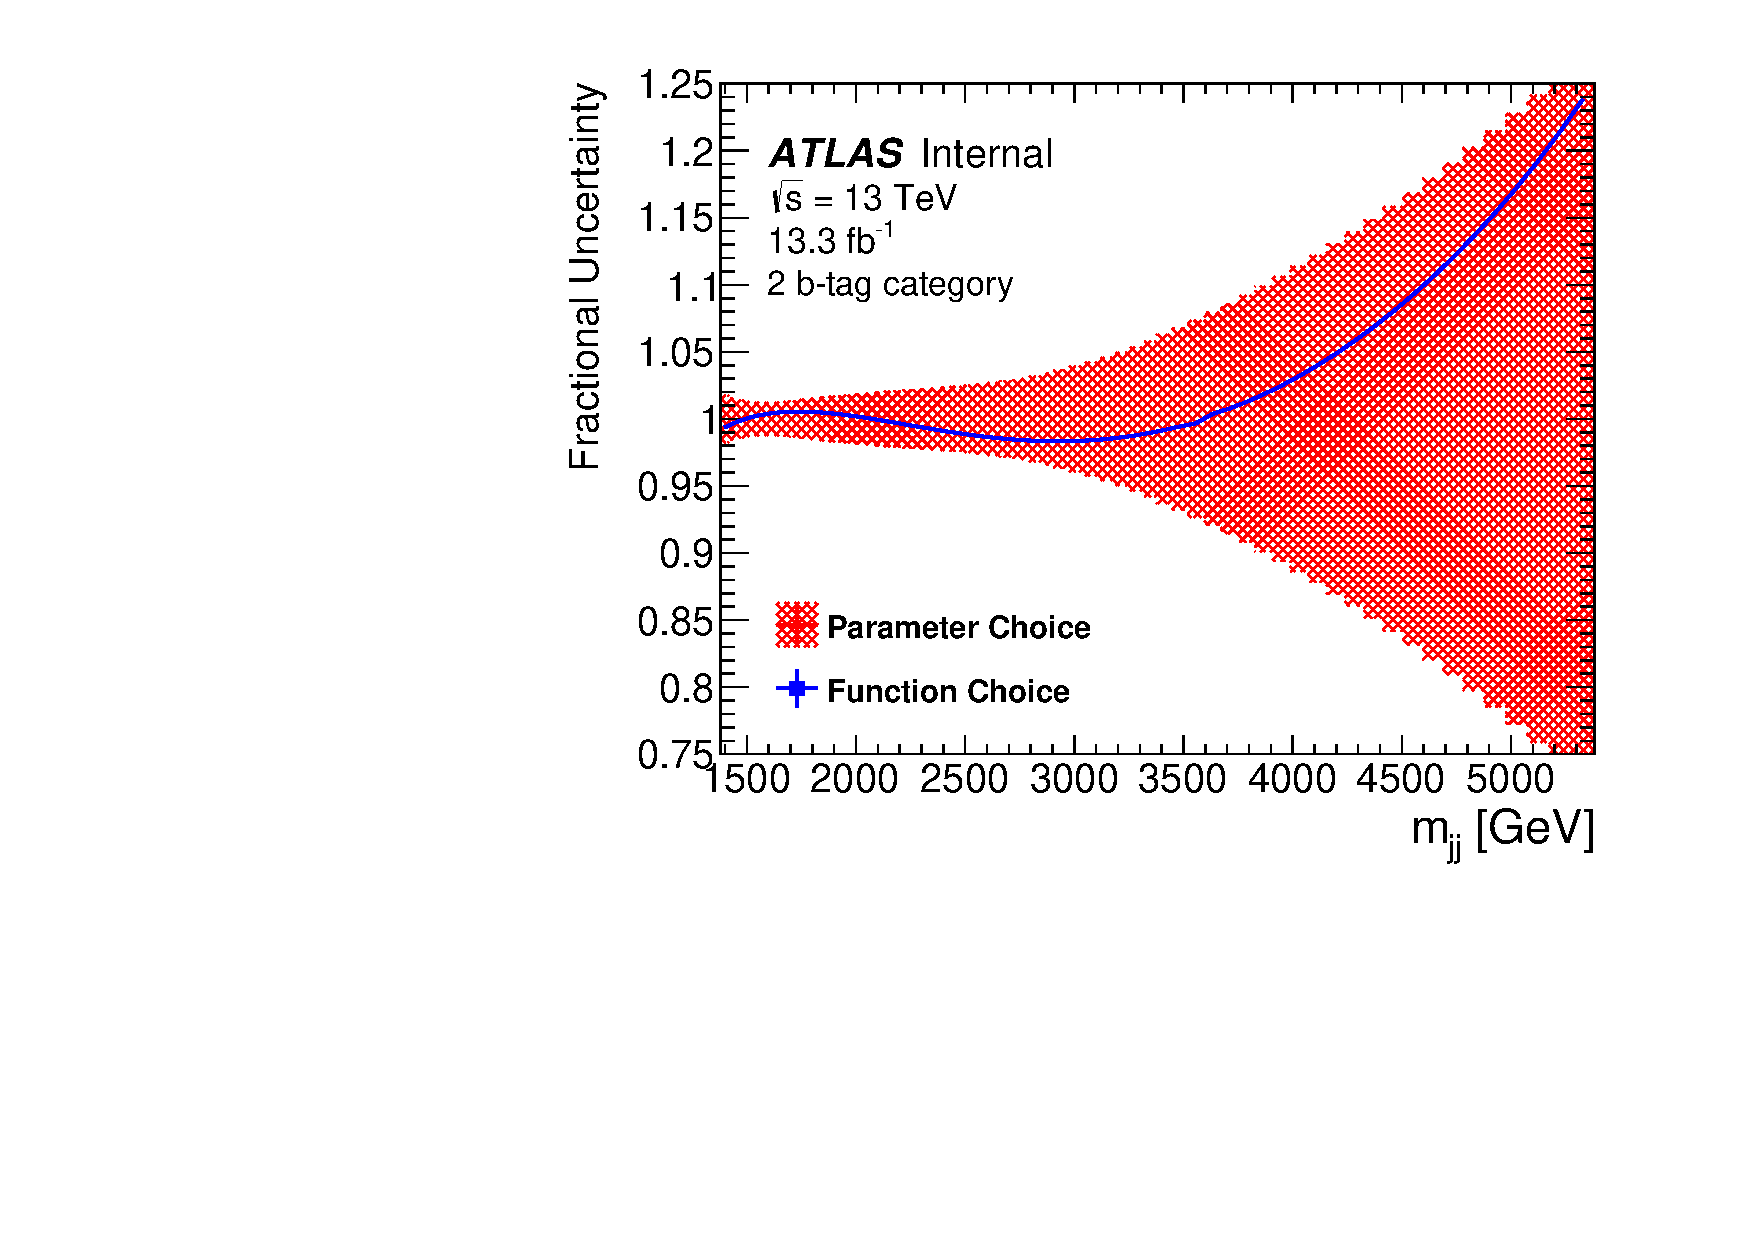
\includegraphics[width=0.47\linewidth, angle=0]{figs/Dibjet/ICHEP/lim-summer_systBkg_bb.pdf}}
    \subcaptionbox{$\geq$1 $b$-tag}{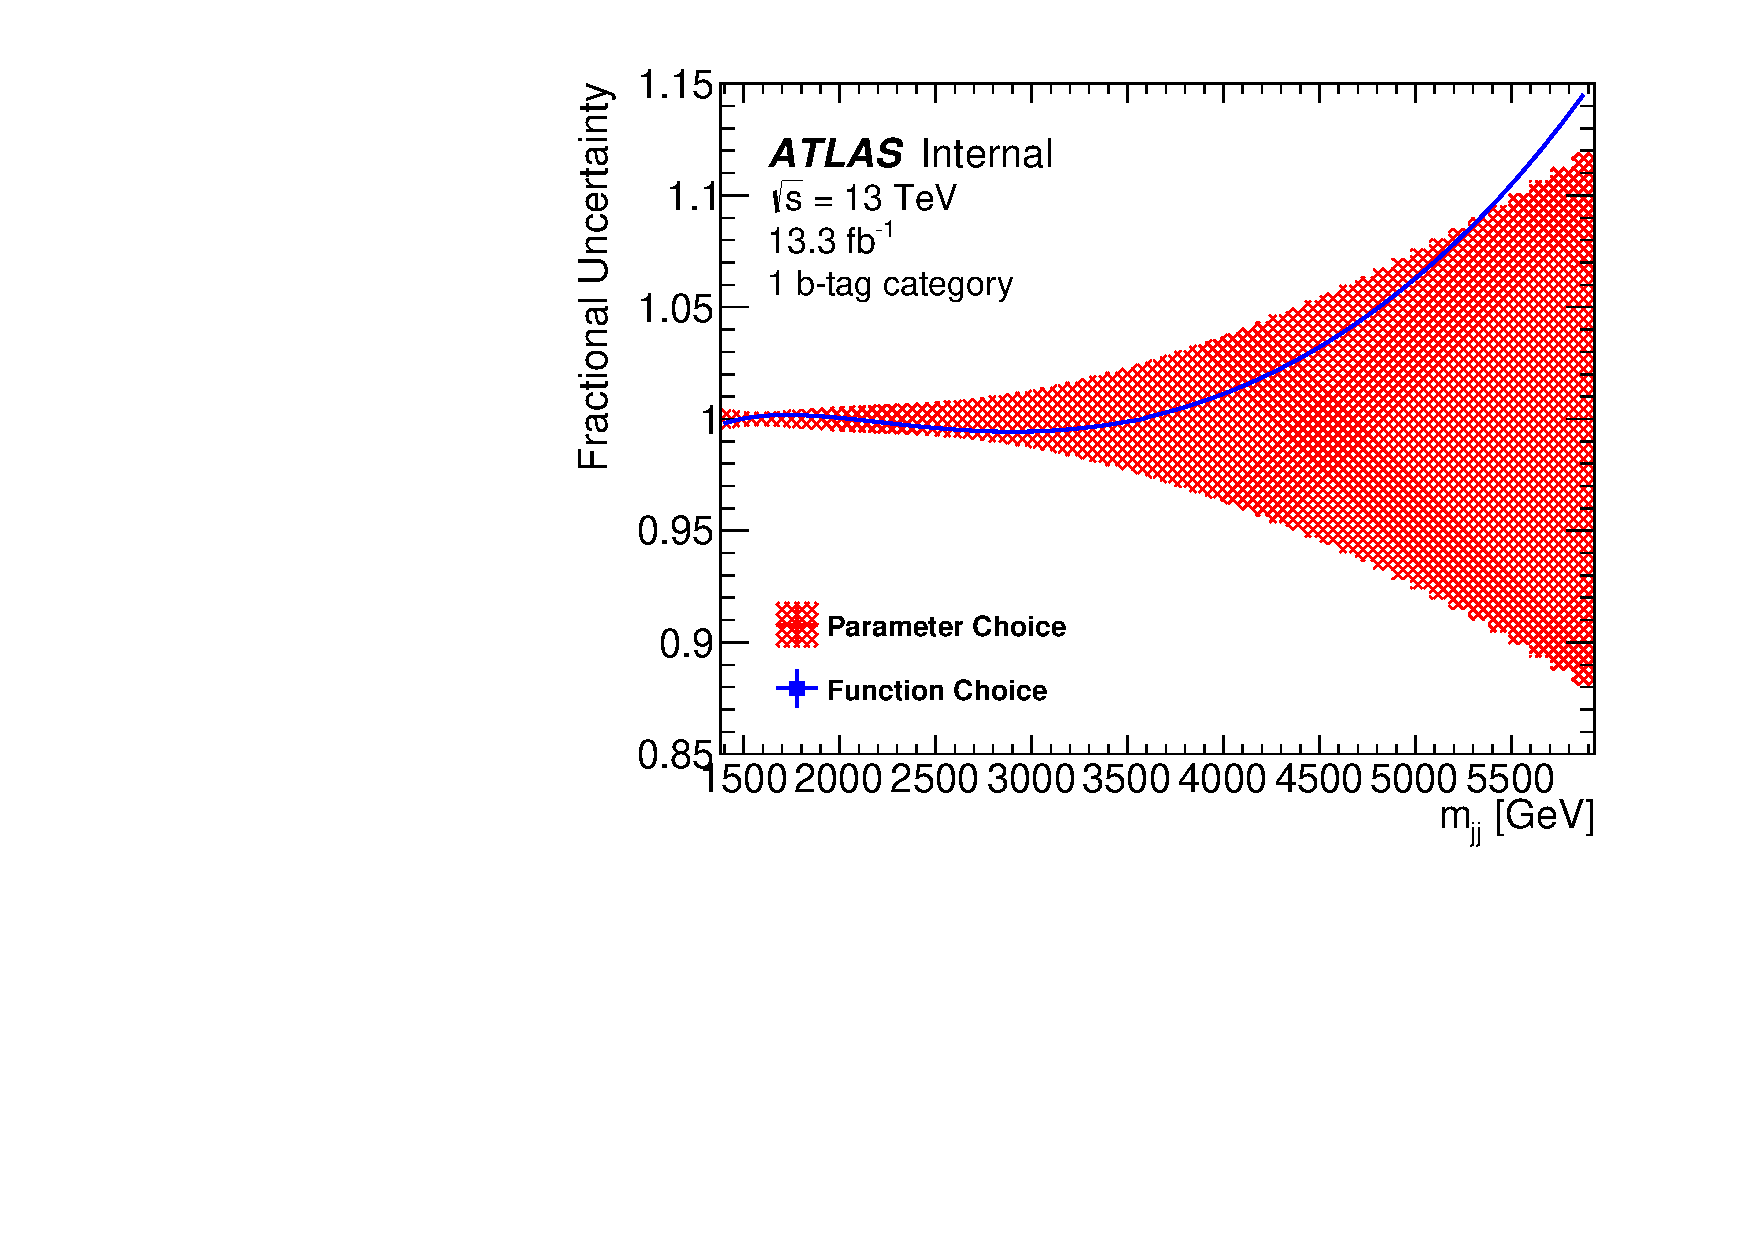
\includegraphics[width=0.47\linewidth, angle=0]{figs/Dibjet/ICHEP/lim-summer_systBkg_b.pdf}}
  \end{center}
  \vspace{-1mm}
  \caption{The background systematic uncertainties for the (a) 2 and (b) $\geq$1 $b$-tag categories
    as a function of dijet invariant mass,~\mjj, for the \textit{Summer16+15} data-set.
    The red shaded region shows the function parameter uncertainty and the
    function choice uncertainty is shown by the blue line. }
  \label{fig:lim-summer_systBkg}
\end{figure}

%Figure~\ref{fig:lim-summer_zprime} and \ref{fig:lim-summer_bstar} show the %% When there was two
Figure~\ref{fig:lim-summer_benchmark} shows the
95\% confidence level upper limits set on $\sigma\,\text{x}\,\mathit{A}\,\text{x}\,\epsilon$
as a function of simulated mass
for the $Z'$-boson and a $b^*$-quark.
%The signal models considered are described in Section~\ref{sec:evt-s+b}.
The observed limit, the expected limit and the 1 and 2 $\sigma$ error bands on the expected limit are shown.
The $\geq1$ $b$-tag category is used for the $b^*$-quark model
and the 2 $b$-tag category is used for the $Z'$-boson models
as these categories provide the strongest limits on the models.
Overlaid are theoretical predictions of
$\sigma\,\text{x}\,\mathit{A}\,\text{x}\,\epsilon$ for the benchmark models described in Section~\ref{sec:evt-s+b}.

%\begin{figure}[!ht]
%  \centering
%   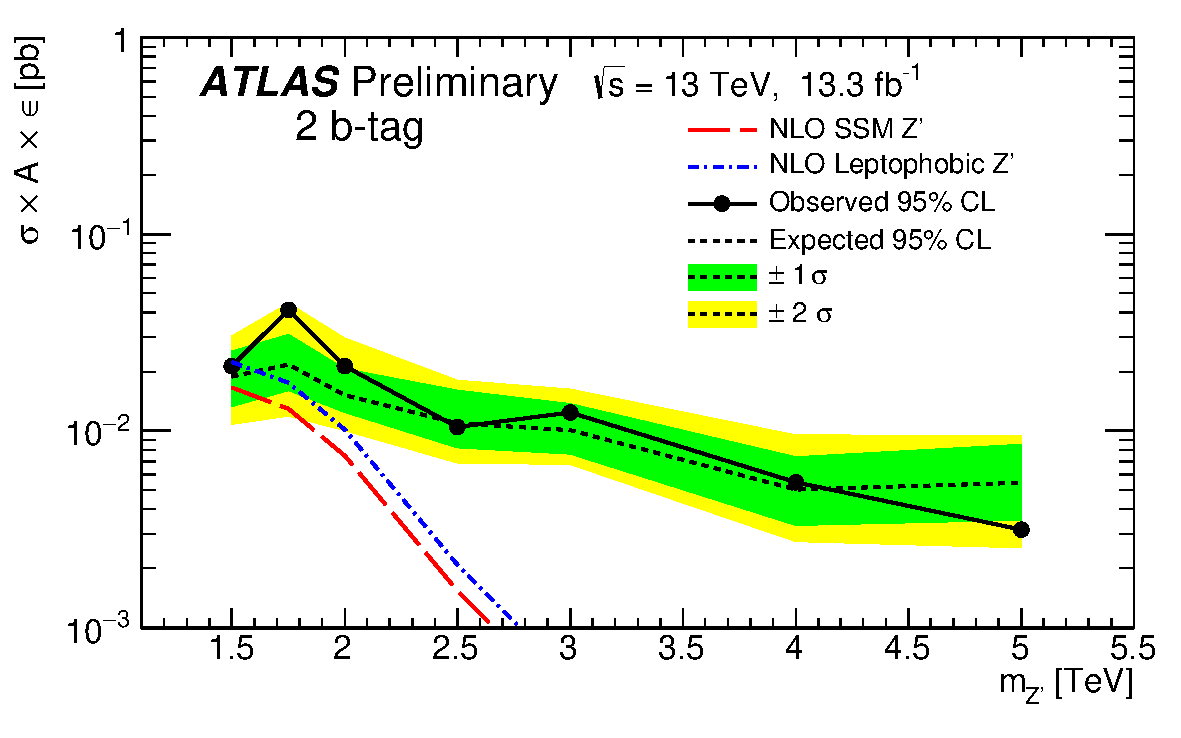
\includegraphics[width=0.7\linewidth, angle=0]{figs/Dibjet/ICHEP/lim-zprime.pdf}
%   \caption[Bayesian 95\% confidence level upper limits on cross-section times acceptance times tagging efficiency
%     for the $Z'$-boson as a function of simulated mass
%     for the 2 $b$-tag category using the \textit{Summer16+15} data-set.
%     The observed limit is shown by the solid black line,
%     the expected limit is shown by the dotted black line
%     and the 1 and 2 $\sigma$ error bands are shown by the green and yellow bands respectively.
%     The theoretical predicition of $\sigma\,\text{x}\,\mathit{A}\,\text{x}\,\epsilon$
%     for the Sequential Standard Model (SSM) and leptophobic $Z'$-boson are overlaid.]
%           {Bayesian 95\% confidence level upper limits on cross-section times acceptance times tagging efficiency
%             for the $Z'$-boson as a function of simulated mass
%             for the 2 $b$-tag category using the \textit{Summer16+15} data-set.
%             The observed limit is shown by the solid black line,
%             the expected limit is shown by the dotted black line
%             and the 1 and 2 $\sigma$ error bands are shown by the green and yellow bands respectively.
%             The theoretical predicition of $\sigma\,\text{x}\,\mathit{A}\,\text{x}\,\epsilon$
%             for the Sequential Standard Model (SSM) and leptophobic $Z'$-boson are overlaid~\cite{dibjet-ichep_conf}.
%           }
%  \label{fig:lim-summer_zprime}
%  \vspace{1cm}
%  \centering
%   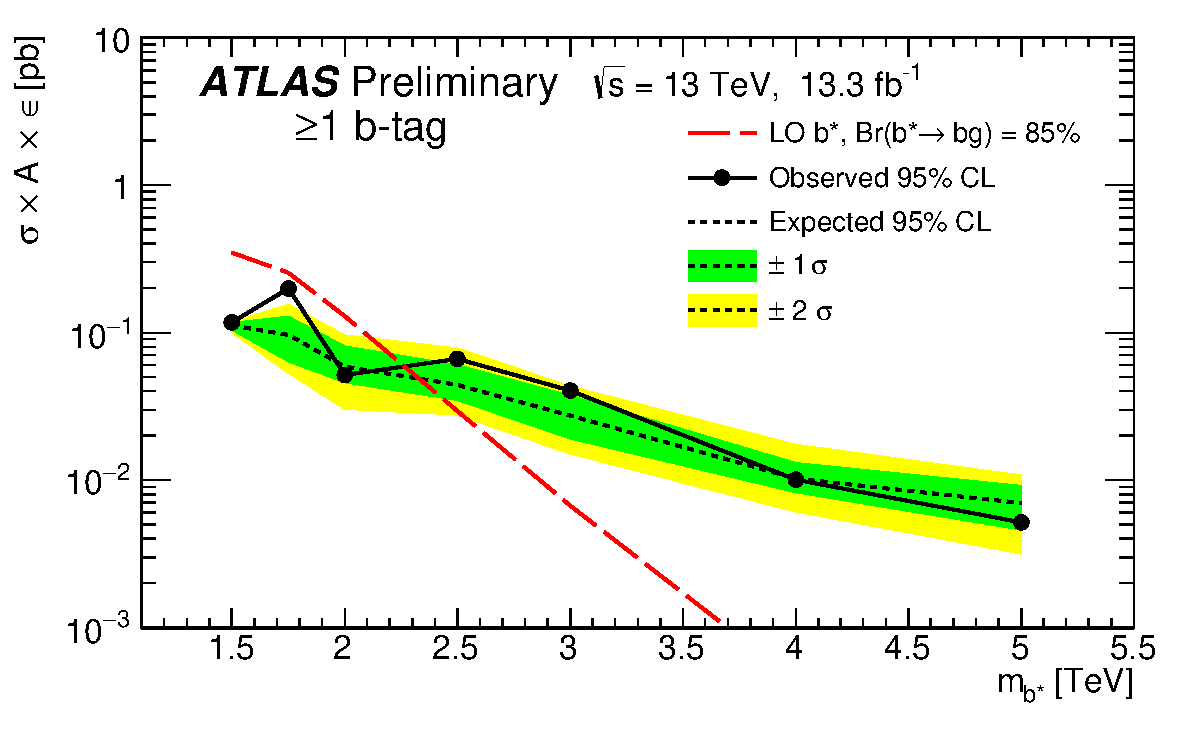
\includegraphics[width=0.7\linewidth, angle=0]{figs/Dibjet/ICHEP/lim-bstar.pdf}
%   \caption[Bayesian 95\% confidence level upper limits on cross-section times acceptance times tagging efficiency
%    for the $b^*$-quark  as a function of simulated mass
%    for the $\geq$1 $b$-tag category using the \textit{Summer16+15} data-set.
%    The observed limit is shown by the solid black line,
%    the expected limit is shown by the dotted black line
%    and the 1 and 2 $\sigma$ error bands are shown by the green and yellow bands respectively.
%    The theoretical predicition of $\sigma\,\text{x}\,\mathit{A}\,\text{x}\,\epsilon$
%    for the $b^*$-quark is overlaid.]
%           {Bayesian 95\% confidence level upper limits on cross-section times acceptance times tagging efficiency
%             for the $b^*$-quark  as a function of simulated mass
%             for the $\geq$1 $b$-tag category using the \textit{Summer16+15} data-set.
%             The observed limit is shown by the solid black line,
%             the expected limit is shown by the dotted black line
%             and the 1 and 2 $\sigma$ error bands are shown by the green and yellow bands respectively.
%             The theoretical predicition of $\sigma\,\text{x}\,\mathit{A}\,\text{x}\,\epsilon$
%             for the $b^*$-quark is overlaid~\cite{dibjet-ichep_conf}.
%           }
%  \label{fig:lim-summer_bstar}
%\end{figure}


\begin{figure}[!ht]
  \centering
  \captionsetup[subfigure]{aboveskip=0pt,justification=centering}
  \subcaptionbox{$Z'$-boson,\hspace{1mm} 2 $b$-tag}{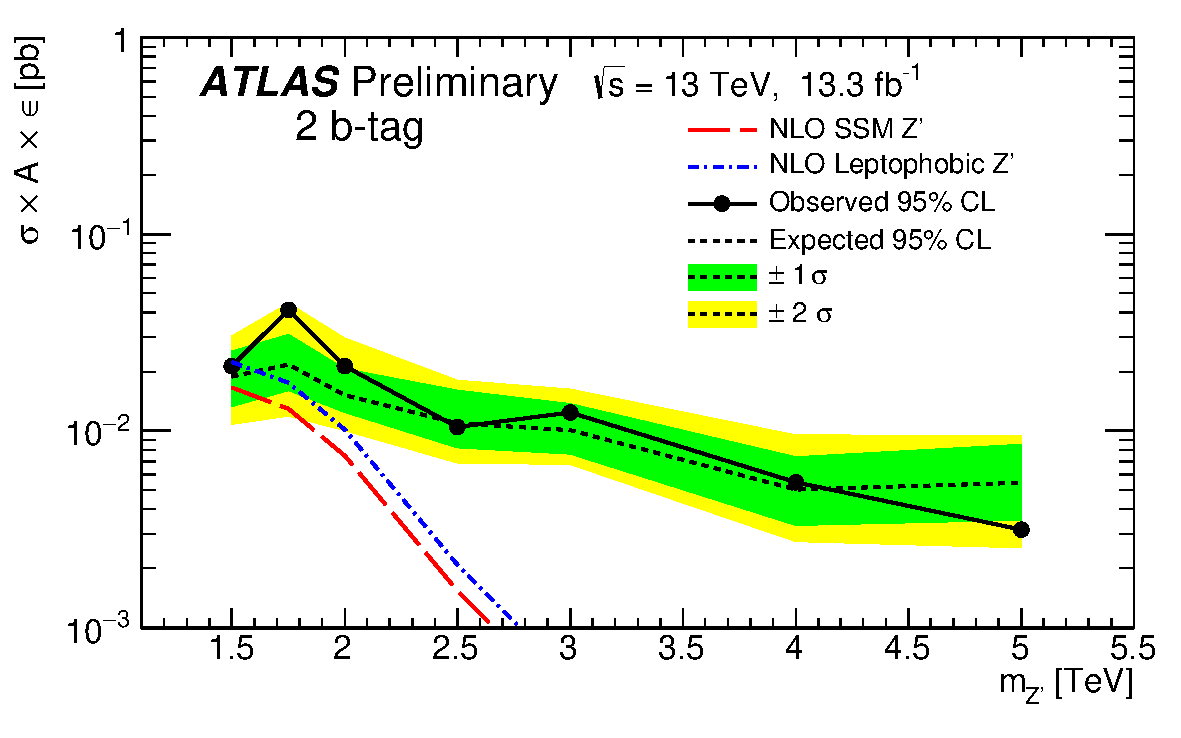
\includegraphics[width=0.8\linewidth, angle=0]{figs/Dibjet/ICHEP/lim-zprime.pdf}}
  \hspace{2mm}
  \subcaptionbox{$b^*$ quark,\hspace{1mm} $\geq$1 $b$-tag}{  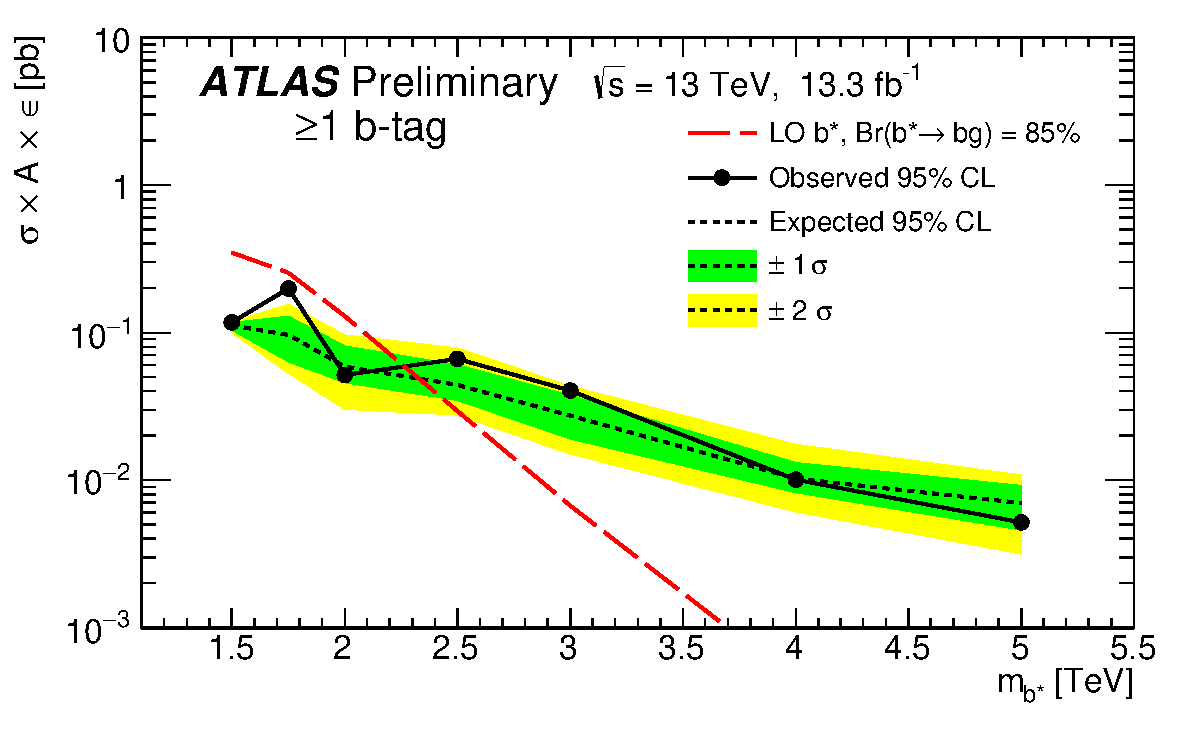
\includegraphics[width=0.8\linewidth, angle=0]{figs/Dibjet/ICHEP/lim-bstar.pdf}}
   \caption[Bayesian 95\% confidence level upper limits on cross-section times acceptance times tagging efficiency
             for the (a) $Z'$-boson and (b) $b^*$-quark  as a function of simulated mass
             using the \textit{Summer16+15} data-set in the 2 and $\geq$1 $b$-tag category respectively.
             The observed limit is shown by the solid black line,
             the expected limit is shown by the dotted black line
             and the 1 and 2 $\sigma$ error bands on the expected limit are shown by the green and yellow bands.
             The theoretical predicition of $\sigma\,\text{x}\,\mathit{A}\,\text{x}\,\epsilon$
             for the Sequential Standard Model (SSM) and leptophobic $Z'$-boson and the $b^*$-quark are overlaid.]
           {Bayesian 95\% confidence level upper limits on cross-section times acceptance times tagging efficiency
             for the (a) $Z'$-boson and (b) $b^*$-quark  as a function of simulated mass
             using the \textit{Summer16+15} data-set in the 2 and $\geq$1 $b$-tag category respectively.
             The observed limit is shown by the solid black line,
             the expected limit is shown by the dotted black line
             and the 1 and 2 $\sigma$ error bands on the expected limit are shown by the green and yellow bands.
             The theoretical predicition of $\sigma\,\text{x}\,\mathit{A}\,\text{x}\,\epsilon$
             for the Sequential Standard Model (SSM) and leptophobic $Z'$-boson and the $b^*$-quark are overlaid~\cite{dibjet-ichep_conf}.
           }
  \label{fig:lim-summer_benchmark}
\end{figure}

The observed and expected limits decrease with increasing simulated mass
due to reduced number of background events at higher mass.
The theoretical $\sigma\,\text{x}\,\mathit{A}\,\text{x}\,\epsilon$ predictions
decrease rapidly as mass increases, due to a combination of
lower signal acceptance times efficiency at high mass, as shown in Figures~\ref{fig:evt-ichep_acc},
and a smaller signal cross-section at high mass.
The signal cross-section is smaller at high mass because of PDF and matrix element effects,
similar to those that caused a smaller QCD dijet production at high mass as described in
 Section~\ref{sec:theo-qcd-dijet_features}.

In the mass regions where the theoretical prediction of $\sigma\,\text{x}\,\mathit{A}\,\text{x}\,\epsilon$
is larger than the upper limit, it can be concluded that the model is excluded at the 95\% confidence level.
Using the \verb|Summer16+15| data-set:
the \mbox{$b^*$-quark} is excluded in the mass range of 1.38 - 2.3 TeV,
the SSM $Z'$-boson cannot be excluded,
and the leptophobic $Z'$-boson is excluded at a mass of 1.5 TeV.

\FloatBarrier

For the generic Gaussian limit setting procedure,
a signal template with a Gaussian shape in dijet invariant mass is used.
The Gaussian shapes are centered on a range of masses
and the width of the considered Gaussians are
15\%, 10\% and 7\% of the simulated mass
in addition to a Gaussian with the width of the detector mass resolution.
The detector mass resolution has been estimated
at previous dijet searches~\cite{dijet-mori16_paper}
and varies from 3\% at 1.5 TeV to 2\% at 5 TeV.
%The dijet mass resolution is defined as the width of a Gaussian fit to mreco/mtruth
% for matched leading and subleading jets divided by the mean of the gaussian.
For the Gaussian limit setting
systematic uncertainties come from the luminosity uncertainty,
the background modelling uncertainties,
and an additional 10\% flat uncertainty to
incorporate sources of systematic uncertainties related to signal modeling
\textbf{LM question. Why 10\%? Much less than the other signal models}.

Figure~\ref{fig:lim-summer_gauss} shows the observed 95\% confidence upper limits
on the product of cross-section, detector acceptance, tagging efficiency and branching ratio,
$\sigma\,\text{x}\,\mathit{A}\,\text{x}\,\epsilon\,\text{x}\,\mathit{BR}$,
for the full range of Gaussian signals described above in both $b$-tagging categories.
For the \verb|Summer16+15| an upper limit is placed on a generic Gaussian signal
ranging from 0.2 to 0.001 pb is set in the mass range 1.4 to 6 TeV.

\begin{figure}[!ht]
  \begin{center}
    \captionsetup[subfigure]{aboveskip=0pt,justification=centering}
   \subcaptionbox{2 $b$-tag}      {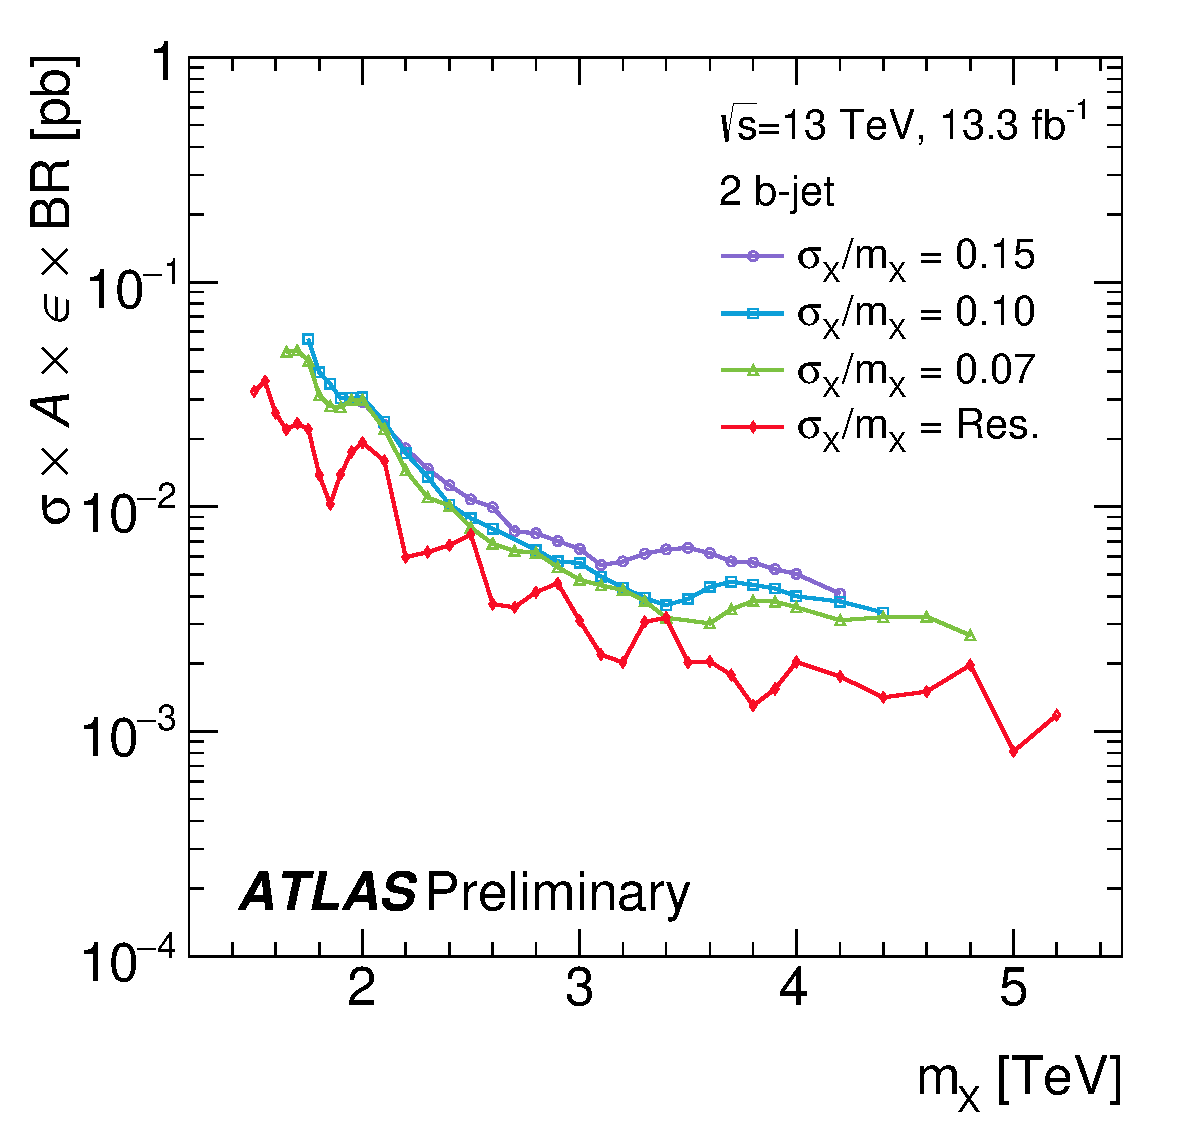
\includegraphics[width=0.47\linewidth, angle=0]{figs/Dibjet/ICHEP/lim-summer_gauss_bb.pdf}}
   \subcaptionbox{$\geq$1 $b$-tag}{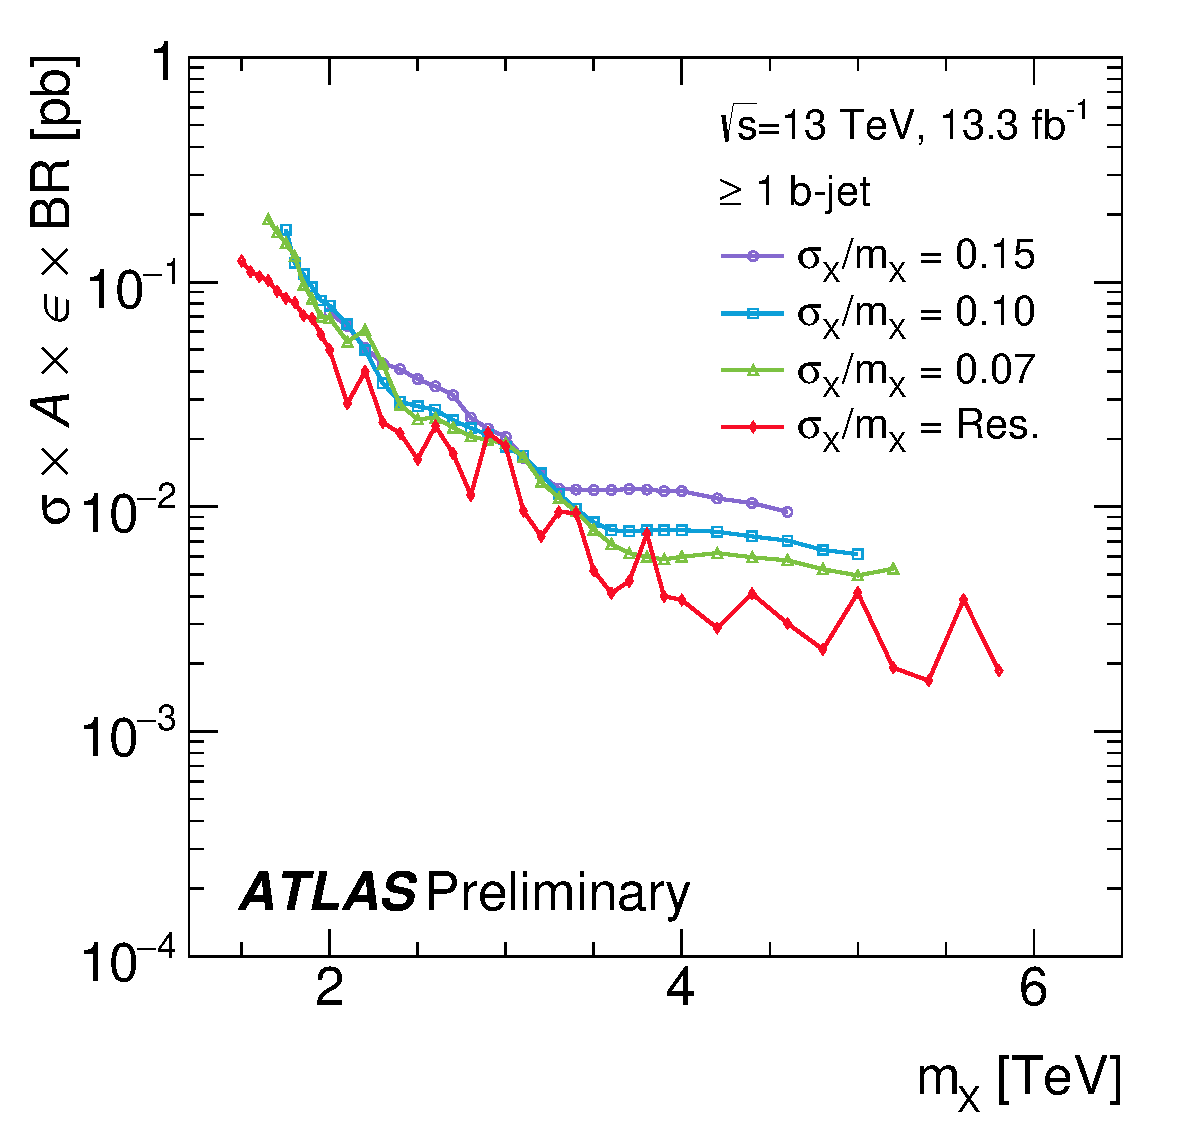
\includegraphics[width=0.47\linewidth, angle=0]{figs/Dibjet/ICHEP/lim-summer_gauss_b.pdf}}
  \end{center}
  \caption[95\% confidence observed upper limits
    on the product of cross-section, detector acceptance, tagging efficiency and branching ratio,
    $\sigma\,\text{x}\,\mathit{A}\,\text{x}\,\epsilon\,\text{x}\,\mathit{BR}$,
    for Gaussian signals for both $b$-tagging categories using the \textit{Summer16+15} data-set.
    The Gaussian widths considered are 15\%, 10\% and 7\% of the simulated mass
    in addition to a Gaussian with the width of the detector mass resolution.]
  {95\% confidence observed upper limits
    on the product of cross-section, detector acceptance, tagging efficiency and branching ratio,
    $\sigma\,\text{x}\,\mathit{A}\,\text{x}\,\epsilon\,\text{x}\,\mathit{BR}$,
    for Gaussian signals for both $b$-tagging categories using the \textit{Summer16+15} data-set.
    The Gaussian widths considered are 15\%, 10\% and 7\% of the simulated mass
    in addition to a Gaussian with the width of the detector mass resolution~\cite{dibjet-ichep_conf}.
  }
  \label{fig:lim-summer_gauss}
\end{figure}

\FloatBarrier

\section{Limits: 2016\_Full}
\label{sec:lim-full}

To do... 
